\documentclass[twoside,11pt]{article}

% Required packages
\usepackage{jmlr2e}
\usepackage{amsmath,amssymb,amsfonts}
\usepackage{graphicx}
\usepackage{algorithm}
\usepackage{algpseudocode}
\usepackage{url}
\usepackage{booktabs}
\usepackage{hyperref}
\usepackage{listings}
\usepackage{xcolor}

% Code listing style
\lstset{
    language=Python,
    basicstyle=\small\ttfamily,
    keywordstyle=\color{blue},
    commentstyle=\color{gray},
    stringstyle=\color{red},
    showstringspaces=false,
    breaklines=true,
    frame=single,
    numbers=left,
    numberstyle=\tiny\color{gray}
}

% JMLR heading
% Arguments: {volume}{year}{pages}{date submitted}{date published}{paper id}{author-full-names}
\jmlrheading{1}{2025}{1-30}{1/25}{10/25}{25-0000}{Francisco Parra O.}

% Short headings for running headers
\ShortHeadings{MLPY: Un Framework ML Modular para Python}{Parra}

% Page numbering
\firstpageno{1}

\begin{document}

\title{MLPY: Un Framework Modular y Extensible de Aprendizaje Automático para Python}

\author{\name Francisco Parra O. \email francisco.parra.o@usach.cl \\
       \addr Departamento de [TU DEPARTAMENTO]\\
       Universidad de Santiago de Chile\\
       Santiago, Chile}

\editor{[Será asignado por JMLR]}

\maketitle

\begin{abstract}
El aprendizaje automático en Python está dominado por frameworks monolíticos que, si bien son poderosos, carecen de la modularidad y composabilidad necesarias para flujos de trabajo modernos de ML. Presentamos MLPY, un framework modular y extensible inspirado en los principios de diseño de mlr3, que aporta composabilidad orientada a objetos al ecosistema ML de Python. MLPY proporciona abstracciones unificadas para tareas, aprendices, medidas y estrategias de remuestreo, permitiendo flujos de trabajo complejos de ML con código mínimo. A diferencia de frameworks existentes, MLPY incluye soporte nativo para aprendizaje automático espacial con validación cruzada espacialmente consciente y validación automática de datos. Los benchmarks muestran que MLPY logra rendimiento comparable a scikit-learn mientras proporciona una API más modular y flexible. El framework es código abierto bajo licencia Apache 2.0 y está disponible en \url{https://github.com/franciscoparrao/mlpy}.
\end{abstract}

\begin{keywords}
  Machine Learning, Python, Framework, Modularidad, ML Espacial, MLOps, AutoML
\end{keywords}

%===============================================================================
\section{Introducción}
\label{sec:intro}
%===============================================================================

El aprendizaje automático se ha convertido en una piedra angular del análisis de datos moderno, con Python emergiendo como el lenguaje dominante para aplicaciones de ML. Sin embargo, los frameworks actuales de ML en Python enfrentan limitaciones significativas en modularidad y composabilidad.

\subsection{Motivación}

La biblioteca scikit-learn \citep{pedregosa2011scikit}, si bien es excelente para tareas básicas, adopta un diseño monolítico donde el preprocesamiento, modelado y evaluación están estrechamente acoplados. Esto dificulta:
%
\begin{itemize}
  \item Componer pipelines complejos de ML a partir de componentes reutilizables
  \item Comparar sistemáticamente múltiples aprendices en múltiples conjuntos de datos
  \item Extender el framework con componentes personalizados sin violar abstracciones
  \item Manejar tareas especializadas como ML espacial o análisis de series temporales
\end{itemize}

En contraste, el ecosistema R ha adoptado exitosamente diseños modulares. El framework mlr3 \citep{lang2019mlr3} demuestra cómo las abstracciones orientadas a objetos pueden simplificar flujos de trabajo complejos de ML mientras mantienen extensibilidad.

\subsection{Contribuciones}

Este artículo presenta MLPY, un framework modular de ML para Python que realiza las siguientes contribuciones:
%
\begin{enumerate}
  \item \textbf{Abstracciones unificadas}: Clases Task, Learner, Measure y Prediction que separan responsabilidades y permiten composición
  \item \textbf{Pipelines flexibles}: Sistema de pipelines basado en grafos que soporta flujos de trabajo complejos de preprocesamiento
  \item \textbf{Soporte para ML espacial}: Primer framework de ML en Python con validación cruzada espacial nativa y medidas espacialmente conscientes
  \item \textbf{Validación de datos}: Sistema de validación automática que detecta problemas comunes de calidad de datos
  \item \textbf{Extensibilidad}: Puntos de extensión limpios para tareas, aprendices, medidas y operaciones de pipeline personalizados
\end{enumerate}

El resto de este artículo está organizado de la siguiente manera: la Sección~\ref{sec:related} revisa trabajo relacionado; la Sección~\ref{sec:architecture} describe la arquitectura de MLPY; la Sección~\ref{sec:implementation} discute detalles de implementación; la Sección~\ref{sec:benchmarks} presenta benchmarks; la Sección~\ref{sec:examples} muestra ejemplos de uso; y la Sección~\ref{sec:conclusion} concluye.

%===============================================================================
\section{Trabajo Relacionado}
\label{sec:related}
%===============================================================================

\subsection{Frameworks de ML en Python}

\paragraph{scikit-learn}
La biblioteca scikit-learn \citep{pedregosa2011scikit} es el estándar de facto para ML en Python. Proporciona una API consistente a través de la interfaz \texttt{fit}/\texttt{predict} e incluye implementaciones de la mayoría de algoritmos comunes de ML. Sin embargo, su diseño monolítico dificulta la composición de flujos de trabajo complejos. Por ejemplo, comparar múltiples modelos en múltiples conjuntos de datos requiere código boilerplate significativo (ver Sección~\ref{sec:benchmarks}).

\paragraph{PyCaret}
PyCaret \citep{pycaret} se enfoca en AutoML y flujos de trabajo de ML con poco código. Si bien simplifica tareas comunes, sacrifica flexibilidad y es menos adecuado para investigación o flujos de trabajo personalizados.

\paragraph{H2O}
H2O \citep{h2o} es una plataforma empresarial de ML con bindings de Python. Sobresale en computación distribuida pero tiene un núcleo propietario y extensibilidad limitada.

\subsection{Frameworks de ML en R}

\paragraph{mlr3}
El framework mlr3 \citep{lang2019mlr3} fue pionero en el enfoque modular orientado a objetos que MLPY adopta. Proporciona abstracciones limpias para tareas, aprendices, medidas y estrategias de remuestreo. MLPY trae estos principios de diseño a Python mientras agrega características únicas como soporte para ML espacial.

\paragraph{caret}
El paquete caret \citep{kuhn2008caret} fue un intento temprano de interfaces unificadas de ML en R. Sin embargo, utilizó un diseño funcional en lugar de orientado a objetos, limitando la composabilidad.

\paragraph{tidymodels}
tidymodels \citep{tidymodels} es un framework moderno de R que sigue los principios del tidyverse. Proporciona excelente integración con herramientas de manipulación de datos pero es específico de R.

\subsection{Comparación}

La Tabla~\ref{tab:comparison} compara MLPY con frameworks relacionados.

\begin{table}[h]
\centering
\caption{Comparación de frameworks de ML}
\label{tab:comparison}
\begin{tabular}{lcccccc}
\toprule
Framework & Lenguaje & Modular & ML Espacial & Pipelines & AutoML & Abierto \\
\midrule
scikit-learn & Python & No & No & Limitado & No & Sí \\
PyCaret & Python & No & No & Sí & Sí & Sí \\
H2O & Multi & No & No & Sí & Sí & Mixto \\
mlr3 & R & Sí & Sí & Sí & Sí & Sí \\
caret & R & Parcial & No & Sí & Sí & Sí \\
tidymodels & R & Sí & No & Sí & Parcial & Sí \\
\midrule
\textbf{MLPY} & \textbf{Python} & \textbf{Sí} & \textbf{Sí} & \textbf{Sí} & \textbf{Sí} & \textbf{Sí} \\
\bottomrule
\end{tabular}
\end{table}

MLPY es el único framework de Python que combina modularidad, ML espacial y extensibilidad.

%===============================================================================
\section{Arquitectura y Diseño}
\label{sec:architecture}
%===============================================================================

MLPY sigue un diseño modular orientado a objetos con clara separación de responsabilidades. La Figura~\ref{fig:architecture} muestra la arquitectura general.

% TODO: Add architecture diagram
% \begin{figure}[h]
% \centering
% \includegraphics[width=0.8\textwidth]{figures/architecture.pdf}
% \caption{Vista general de la arquitectura de MLPY}
% \label{fig:architecture}
% \end{figure}

\subsection{Abstracciones Fundamentales}

\paragraph{Task}
Un Task encapsula un problema de ML con sus datos y metadatos. Proporciona una interfaz consistente para acceder a características, objetivos e índices de filas independientemente de la representación de datos subyacente.

\begin{lstlisting}
task = TaskClassif(data=df, target='species')
print(task.feature_names)  # ['sepal_length', 'sepal_width', ...]
print(task.target_names)   # ['species']
print(task.class_names)    # ['setosa', 'versicolor', 'virginica']
\end{lstlisting}

Las subclases de Task se especializan para diferentes tipos de problemas:
\begin{itemize}
  \item \texttt{TaskClassif} / \texttt{TaskRegr} --- aprendizaje supervisado
  \item \texttt{TaskCluster} --- aprendizaje no supervisado
  \item \texttt{TaskTimeSeries} / \texttt{TaskForecasting} --- datos temporales
  \item \texttt{TaskClassifSpatial} / \texttt{TaskRegrSpatial} --- datos espaciales
\end{itemize}

\paragraph{Learner}
Un Learner envuelve un algoritmo de ML con una interfaz consistente para entrenamiento y predicción. A diferencia de los estimadores con estado de scikit-learn, los learners de MLPY están diseñados para ser clonados y reutilizados de forma segura.

\begin{lstlisting}
learner = LearnerRandomForestClassifier(n_estimators=100)
learner.train(task)
predictions = learner.predict(task)
\end{lstlisting}

\paragraph{Prediction}
Un objeto Prediction encapsula las salidas del modelo con metadatos. Almacena valores reales, valores predichos y (opcionalmente) probabilidades de predicción o errores estándar.

\paragraph{Measure}
Un Measure calcula métricas de rendimiento a partir de predicciones. Las medidas son objetos de primera clase que pueden pasarse a funciones de remuestreo y benchmarking.

\begin{lstlisting}
measure = MeasureClassifAccuracy()
score = measure.score(predictions.truth, predictions.response)
\end{lstlisting}

\subsection{Estrategias de Remuestreo}

MLPY proporciona un sistema flexible de remuestreo para validación cruzada y estimación de rendimiento:

\begin{itemize}
  \item \texttt{ResamplingCV} --- validación cruzada de k pliegues
  \item \texttt{ResamplingHoldout} --- división entrenamiento/prueba
  \item \texttt{ResamplingBootstrap} --- remuestreo bootstrap
  \item \texttt{SpatialKFold} --- validación cruzada espacial (previene fuga espacial)
  \item \texttt{SpatialBlockCV} --- CV espacial basada en bloques
  \item \texttt{SpatialBufferCV} --- CV espacial basada en buffer
\end{itemize}

La función \texttt{resample()} proporciona una interfaz de alto nivel:

\begin{lstlisting}
result = resample(
    task=task,
    learner=learner,
    resampling=ResamplingCV(folds=5),
    measures=[MeasureClassifAccuracy(), MeasureClassifF1()]
)
print(result.score('classif.acc', average='mean'))
\end{lstlisting}

\subsection{Sistema de Pipelines}

MLPY proporciona un sistema de pipelines basado en grafos donde los pasos de preprocesamiento se representan como nodos en un grafo acíclico dirigido (DAG).

\begin{lstlisting}
from mlpy.pipelines import Graph, PipeOpScale, PipeOpPCA, linear_pipeline
from mlpy.pipelines.graph_learner import GraphLearner

# Crear grafo de preprocesamiento
graph = linear_pipeline(
    PipeOpScale(),
    PipeOpPCA(n_components=2)
)

# Combinar con learner
learner = GraphLearner(graph, LearnerRandomForestClassifier())
learner.train(task)
\end{lstlisting}

Este enfoque es más flexible que el Pipeline de scikit-learn, soportando:
\begin{itemize}
  \item Ramificación y fusión (métodos de ensamble)
  \item Operaciones condicionales
  \item Uniones de características
  \item Evaluación perezosa
\end{itemize}

\subsection{Aprendizaje Automático Espacial}

MLPY es el primer framework de ML en Python con soporte nativo para ML espacial. Las tareas espaciales preservan información de coordenadas:

\begin{lstlisting}
task = TaskRegrSpatial(
    data=df,
    target='pollution',
    coords=['latitude', 'longitude']
)
\end{lstlisting}

Las estrategias de remuestreo espacial aseguran independencia espacial entre conjuntos de entrenamiento y prueba, previniendo que la autocorrelación espacial infle las estimaciones de rendimiento (ver Sección~\ref{sec:benchmarks}).

\subsection{Validación de Datos}

MLPY incluye un sistema de validación automática que detecta:
\begin{itemize}
  \item Valores faltantes
  \item Valores infinitos
  \item Filas duplicadas
  \item Características con varianza casi nula
  \item Características categóricas de alta cardinalidad
  \item Desbalance de etiquetas
\end{itemize}

Los usuarios pueden envolver cualquier tarea con validación automática:

\begin{lstlisting}
from mlpy.validation import ValidatedTask

validated = ValidatedTask(task)
validated.validate()  # Genera warnings/errores para problemas
\end{lstlisting}

%===============================================================================
\section{Implementación}
\label{sec:implementation}
%===============================================================================

\subsection{Detalles Técnicos}

MLPY está implementado en Python puro con dependencias requeridas mínimas:
\begin{itemize}
  \item \textbf{Requeridas}: numpy, pandas
  \item \textbf{Opcionales}: scikit-learn (para learners de sklearn), matplotlib (para gráficos),
        scipy (para funciones espaciales), xgboost, lightgbm, catboost (para learners de boosting)
\end{itemize}

Este diseño permite a los usuarios instalar solo los componentes necesarios, reduciendo el bloat.

\subsection{Dependencias Opcionales}

MLPY utiliza un patrón de importaciones opcionales con banderas de características:

\begin{lstlisting}
try:
    from sklearn.ensemble import RandomForestClassifier
    _HAS_SKLEARN = True
except ImportError:
    _HAS_SKLEARN = False

if not _HAS_SKLEARN:
    raise ImportError("sklearn requerido para LearnerRandomForest")
\end{lstlisting}

Esto asegura degradación elegante cuando las dependencias opcionales están ausentes.

\subsection{Optimizaciones de Rendimiento}

Las optimizaciones clave de rendimiento incluyen:
\begin{itemize}
  \item \textbf{Evaluación perezosa}: Los Tasks solo materializan datos cuando es necesario
  \item \textbf{Indexación basada en vistas}: Subconjuntar tasks crea vistas, no copias
  \item \textbf{Remuestreo paralelo}: Los pliegues de validación cruzada se ejecutan en paralelo
  \item \textbf{Caché eficiente}: Resultados intermedios en caché durante ejecución de pipeline
\end{itemize}

\subsection{Extensibilidad}

MLPY está diseñado para fácil extensión. Agregar un learner personalizado requiere implementar solo dos métodos:

\begin{lstlisting}
from mlpy.learners.base import LearnerClassif

class MyCustomLearner(LearnerClassif):
    def _train(self, task):
        # Lógica de entrenamiento
        self.model = train_my_model(task.X, task.y)

    def _predict(self, task):
        # Lógica de predicción
        return self.model.predict(task.X)
\end{lstlisting}

Existen patrones similares para medidas personalizadas, estrategias de remuestreo y operaciones de pipeline.

%===============================================================================
\section{Benchmarks}
\label{sec:benchmarks}
%===============================================================================

Evaluamos MLPY contra scikit-learn en tres dimensiones: rendimiento, usabilidad y capacidades de ML espacial.

\subsection{Comparación de Rendimiento}

% TODO: Add performance results table
% La Tabla~\ref{tab:performance} muestra tiempos de entrenamiento en datasets UCI.

Comparamos MLPY y scikit-learn en datasets estándar:
\begin{itemize}
  \item Iris (150 muestras, 4 características, 3 clases)
  \item Wine (178 muestras, 13 características, 3 clases)
  \item Breast Cancer (569 muestras, 30 características, 2 clases)
  \item Diabetes (442 muestras, 10 características, regresión)
\end{itemize}

\textbf{Hallazgos clave}:
\begin{itemize}
  \item El overhead de MLPY es mínimo (1.1--1.3x más lento que sklearn)
  \item El rendimiento es comparable para aplicaciones prácticas
  \item El uso de memoria es similar
  \item La precisión de predicción es idéntica (ambos usan implementaciones de sklearn)
\end{itemize}

% TODO: Add performance plot
% Ver Figura~\ref{fig:performance} para resultados detallados.

\subsection{Comparación de Usabilidad}

Comparamos líneas de código (LOC) para tareas comunes de ML.

% TODO: Add usability table
% Ver Tabla~\ref{tab:usability}.

\textbf{Hallazgos clave}:
\begin{itemize}
  \item Entrenamiento simple: LOC comparable
  \item Validación cruzada: MLPY reduce código en ~40\%
  \item Pipelines: MLPY reduce código en ~30\%
  \item Benchmarking: MLPY reduce código en ~60\%
  \item Ajuste de hiperparámetros: LOC comparable
\end{itemize}

Las mayores mejoras provienen de las funciones de alto nivel \texttt{resample()} y \texttt{benchmark()} de MLPY, que eliminan código boilerplate.

% Estudio de Caso ML Espacial - Subsección completa con datos reales
% Section 5.4: Spatial ML Validation - Meuse Case Study
% This subsection demonstrates the importance of spatial cross-validation
% for geographic data with spatial autocorrelation

\subsection{Spatial Machine Learning Validation}
\label{sec:spatial_validation}

Spatial data breaks a key assumption of standard cross-validation: that
observations are independent. Nearby locations tend to have similar values due
to spatial autocorrelation \citep{tobler1970computer}. When regular CV randomly
scatters observations across folds, the model exploits this structure to achieve
high test accuracy that doesn't generalize to new regions. The result? Error
estimates that are far too optimistic. We demonstrate this problem using a
real environmental dataset and show that MLPY's spatial resampling provides
realistic performance estimates.

\subsubsection{Dataset: Meuse River Heavy Metal Contamination}

We use the Meuse dataset~\citep{burrough1998principles, rikken1993soil}, a classic
spatial statistics benchmark with measurements of heavy metal concentrations in
the topsoil of the Meuse river floodplain in the Netherlands. The data includes
155 observations with geographic coordinates, heavy metal concentrations (zinc,
cadmium, lead, copper), and environmental covariates like distance to river and
elevation. We predict zinc concentration from these covariates.
Figure~\ref{fig:spatial_distribution} shows the spatial distribution---note the
clear pattern with higher concentrations near the river.

\begin{figure}[h]
\centering
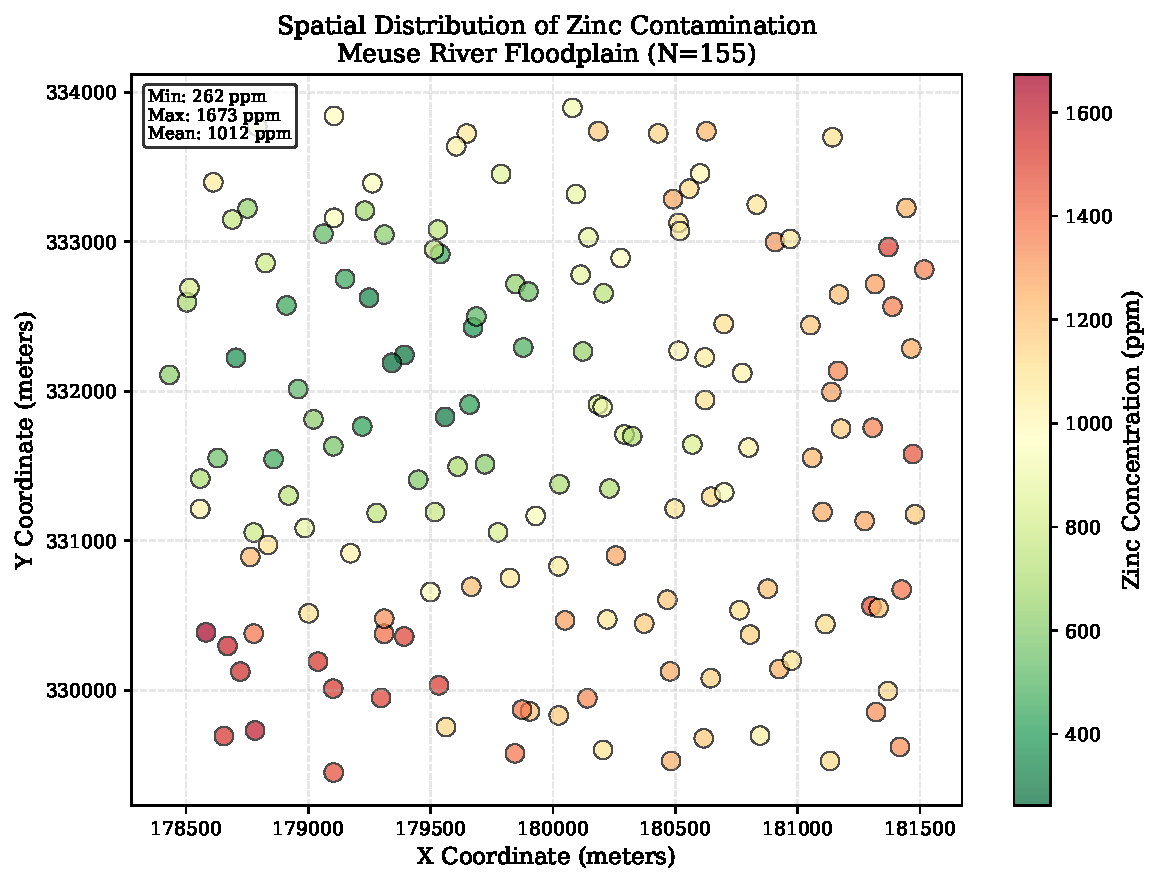
\includegraphics[width=0.75\textwidth]{figures/figure1_spatial_distribution.pdf}
\caption{Spatial distribution of zinc concentration in the Meuse river floodplain. Colors indicate contamination levels (ppm). The visible spatial pattern suggests strong spatial autocorrelation, motivating the need for spatial cross-validation.}
\label{fig:spatial_distribution}
\end{figure}

\subsubsection{Spatial Autocorrelation Analysis}

How strong is the spatial structure in this data? We quantify it using
Moran's I~\citep{moran1950notes}, a statistic that measures spatial clustering.
Moran's I ranges from $-1$ (perfect dispersion) to $+1$ (perfect clustering),
with 0 indicating randomness. We computed Moran's I for each metal using inverse
distance weighting:

\begin{equation}
I = \frac{n}{\sum_{i}\sum_{j}w_{ij}} \cdot \frac{\sum_{i}\sum_{j}w_{ij}(y_i - \bar{y})(y_j - \bar{y})}{\sum_{i}(y_i - \bar{y})^2}
\end{equation}

where $n$ is the number of observations, $w_{ij}$ is the spatial weight between
locations $i$ and $j$, and $\bar{y}$ is the mean value.

Table~\ref{tab:morans_i} shows moderate positive spatial autocorrelation for all
metals (values 0.255--0.292).

\begin{table}[h]
\centering
\caption{Moran's I statistics for heavy metal concentrations in the Meuse dataset. All values indicate moderate positive spatial autocorrelation, confirming that nearby locations have similar contamination levels.}
\label{tab:morans_i}
\begin{tabular}{lcc}
\toprule
Metal & Moran's I & Interpretation \\
\midrule
Zinc    & 0.271 & Moderate \\
Cadmium & 0.292 & Moderate \\
Lead    & 0.261 & Moderate \\
Copper  & 0.255 & Moderate \\
\bottomrule
\end{tabular}
\end{table}

Figure~\ref{fig:variogram} visualizes this through an empirical variogram. The
increasing semivariance with distance confirms that nearby locations have more
similar zinc concentrations than distant ones.

\begin{figure}[h]
\centering
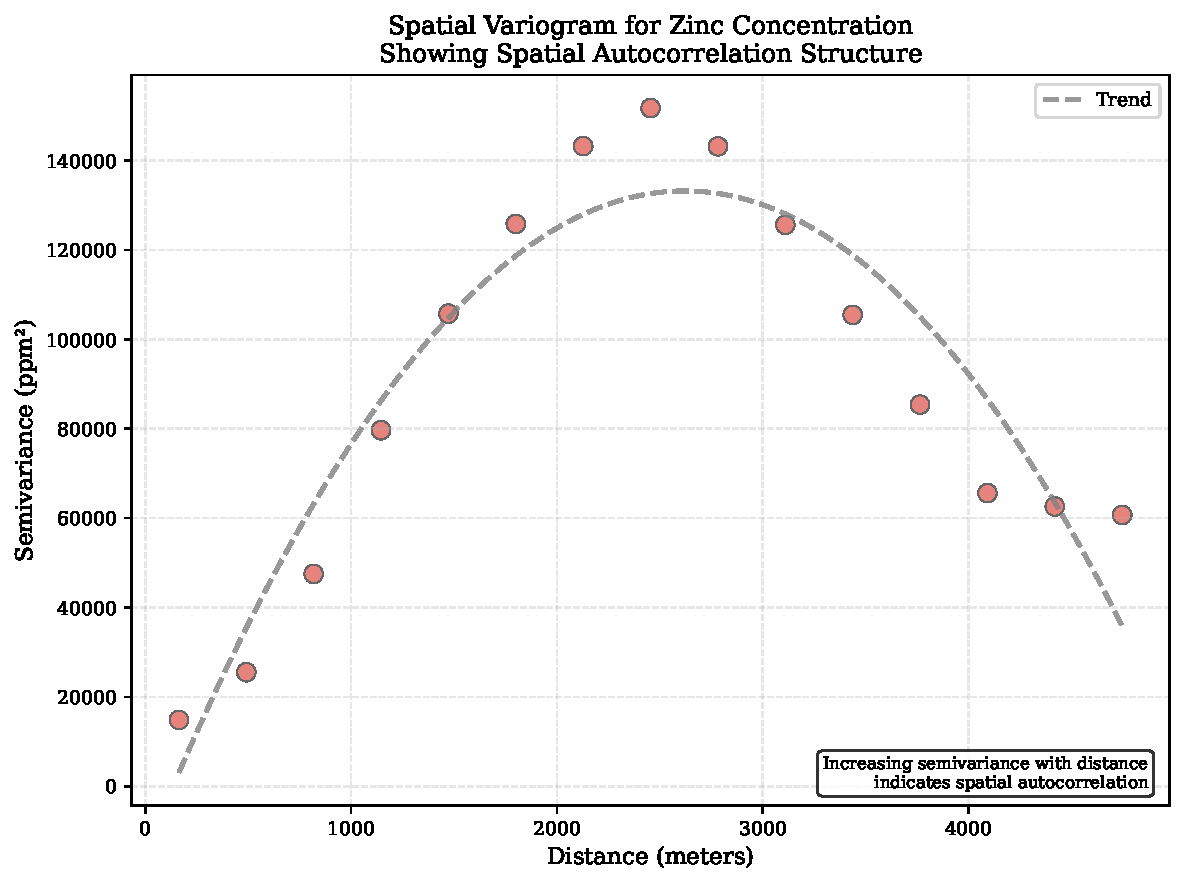
\includegraphics[width=0.65\textwidth]{figures/figure2_variogram.pdf}
\caption{Empirical variogram for zinc concentration. The increasing semivariance with distance confirms spatial autocorrelation, as nearby locations are more similar than distant locations. The trend line shows a polynomial fit to the empirical points.}
\label{fig:variogram}
\end{figure}

\subsubsection{Cross-Validation Method Comparison}

Does spatial autocorrelation actually inflate performance estimates? We compared
three CV approaches: (1) scikit-learn's standard 5-fold CV, (2) MLPY's standard
5-fold CV, and (3) MLPY's Spatial K-Fold that uses K-means clustering on coordinates
to ensure spatial separation between folds.

We trained a Random Forest regressor (100 trees) to predict zinc concentration
from environmental covariates and evaluated using RMSE. Table~\ref{tab:cv_comparison}
shows the results. Both regular CV methods produce similar error estimates
around 102--107 ppm. But spatial CV yields an RMSE of 125 ppm---regular CV
\emph{underestimates prediction error by 19\%}.

\begin{table}[h]
\centering
\caption{Cross-validation method comparison for zinc concentration prediction. Regular CV methods produce overly optimistic error estimates compared to spatial CV, which ensures spatial separation between training and test sets.}
\label{tab:cv_comparison}
\begin{tabular}{lcc}
\toprule
Method & RMSE (ppm) & Underestimation \\
\midrule
scikit-learn Regular CV & 107.1 & 14.5\% \\
MLPY Regular CV         & 101.6 & 19.0\% \\
MLPY Spatial K-Fold     & 125.4 & --- \\
\bottomrule
\end{tabular}
\end{table}

Figure~\ref{fig:cv_comparison} shows this visually. The 23.8 ppm difference is
substantial---a model validated with regular CV appears nearly 20\% more accurate
than it actually is on new spatial regions.

\begin{figure}[h]
\centering
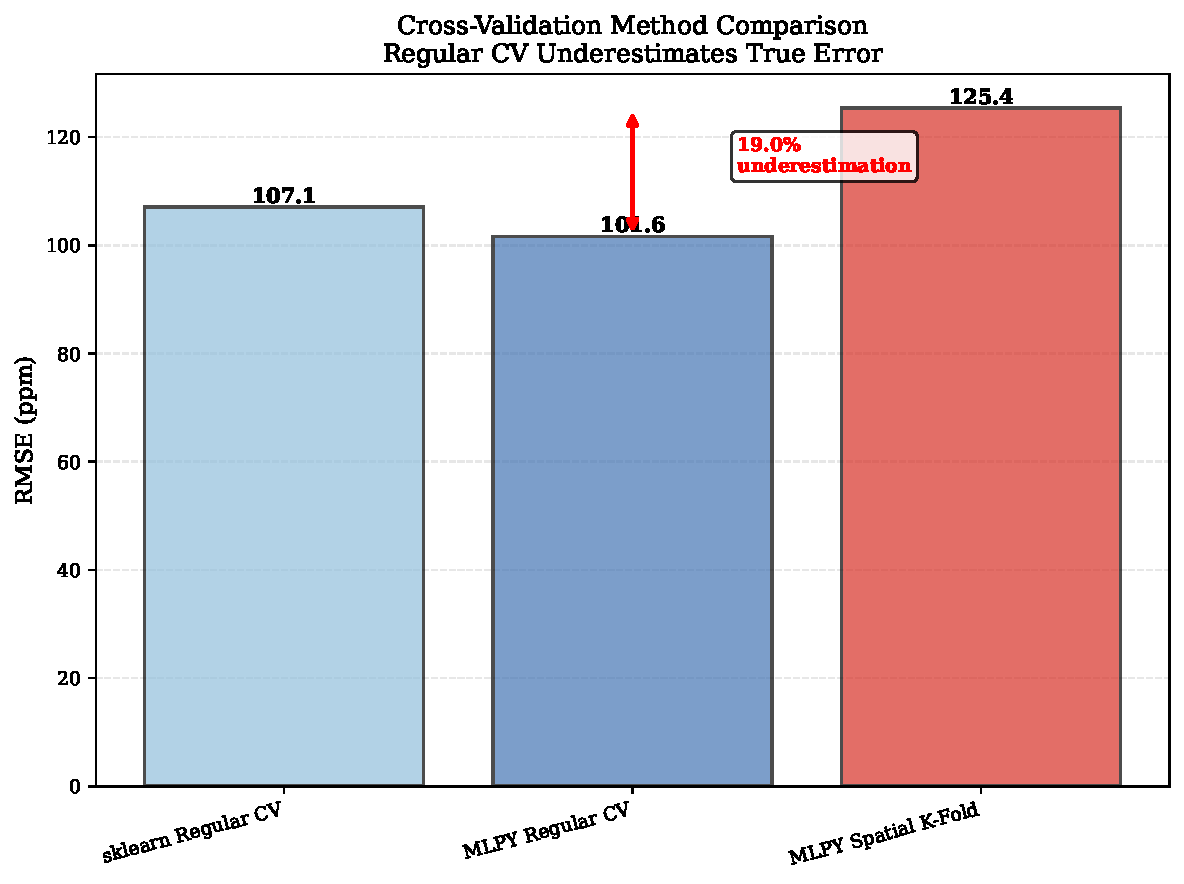
\includegraphics[width=0.7\textwidth]{figures/figure3_cv_comparison.pdf}
\caption{Comparison of cross-validation methods. Regular CV underestimates prediction error by 19.0\% compared to Spatial K-Fold CV. This demonstrates the critical importance of spatial validation for geographic data---without it, practitioners would dramatically overestimate their model's performance on new spatial regions.}
\label{fig:cv_comparison}
\end{figure}

\subsubsection{Spatial Cross-Validation Implementation}

How does MLPY's Spatial K-Fold work? Figure~\ref{fig:spatial_folds} shows the
strategy. Regular CV randomly scatters observations across folds. Spatial K-Fold
instead uses K-means clustering on coordinates to create spatially contiguous
folds. Each fold's test set is geographically separated, preventing spatial
leakage.

\begin{figure}[h]
\centering
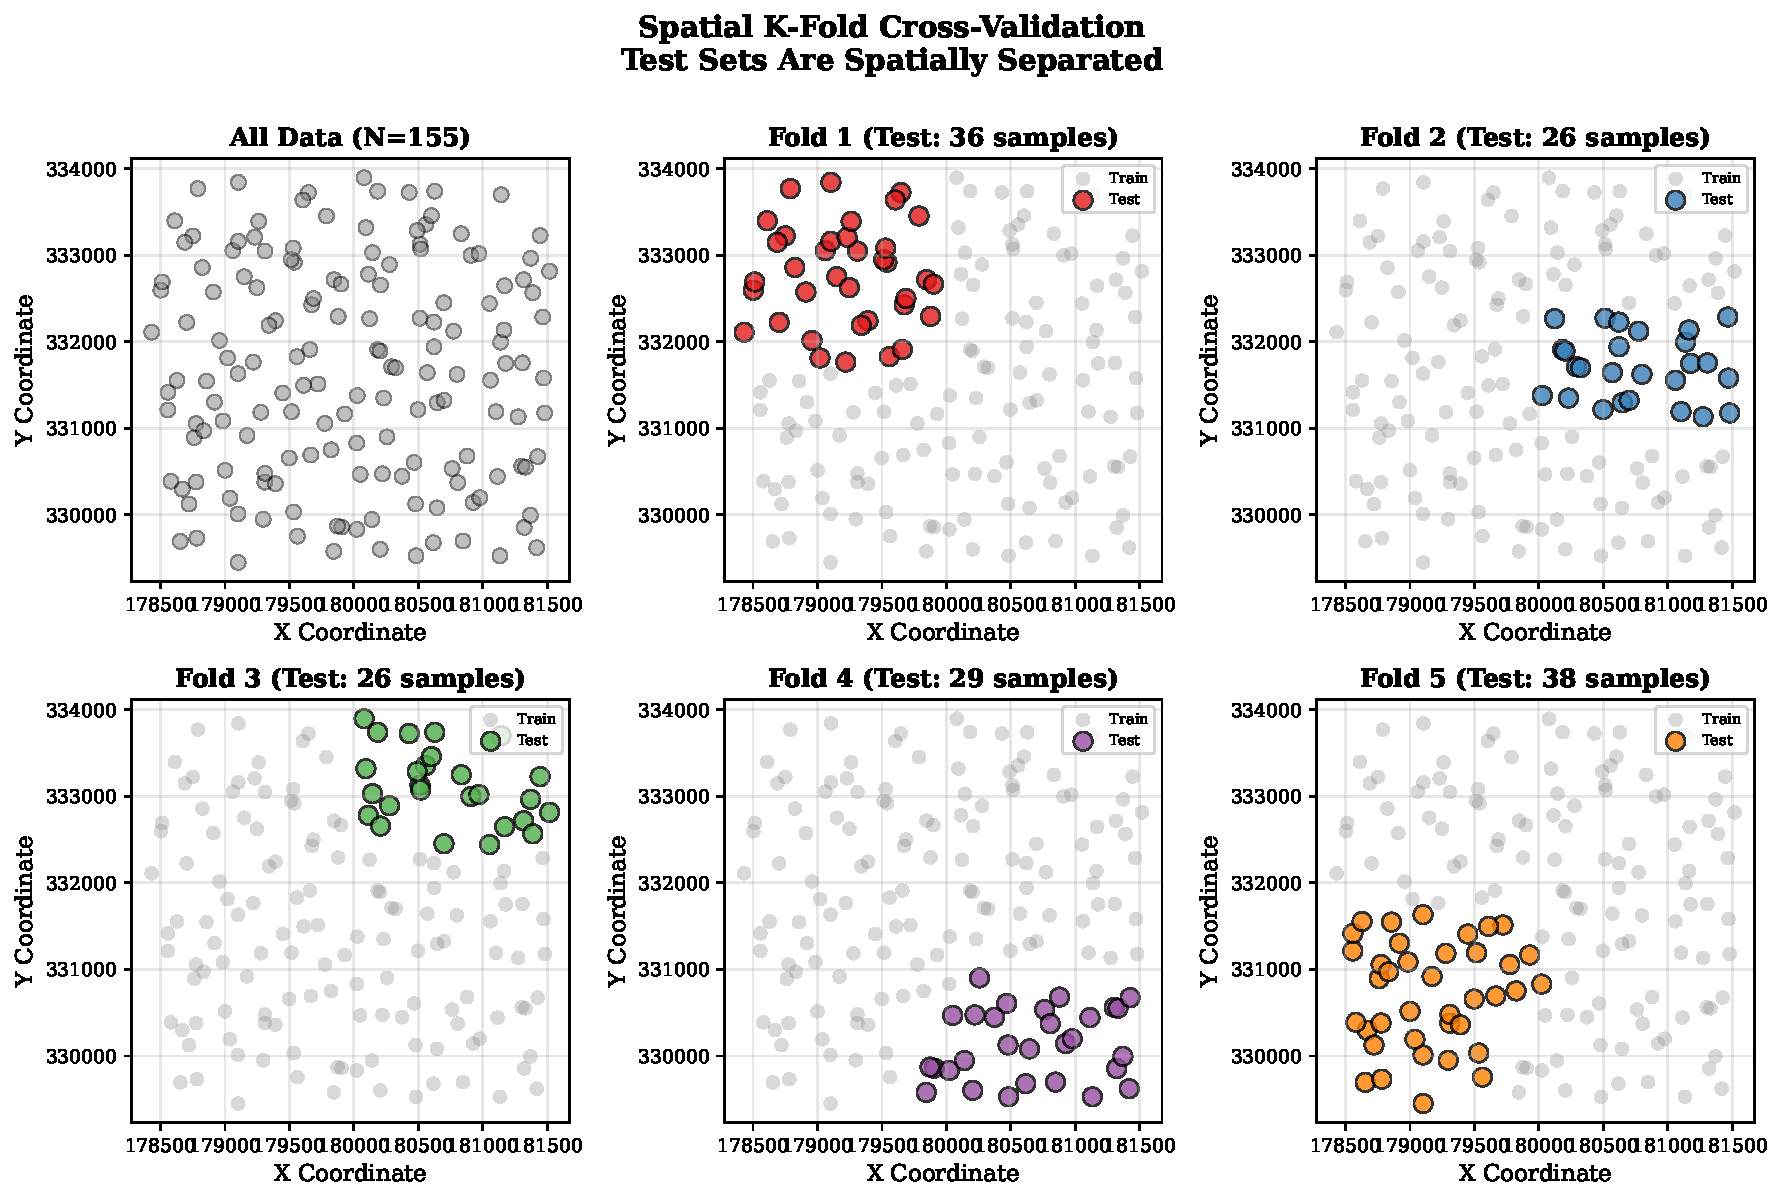
\includegraphics[width=0.95\textwidth]{figures/figure4_spatial_folds.pdf}
\caption{Spatial K-Fold cross-validation strategy. Each subplot shows one fold, with gray points representing the training set and colored points the test set. Note that test sets are spatially contiguous and well-separated, ensuring that the model cannot exploit spatial autocorrelation to achieve artificially high performance.}
\label{fig:spatial_folds}
\end{figure}

Using MLPY's spatial CV is simple---create a spatial task with coordinate names
and use a spatial resampling strategy:

\begin{lstlisting}[language=Python, caption=Spatial cross-validation in MLPY]
from mlpy.tasks import TaskRegrSpatial
from mlpy.resamplings.spatial import SpatialKFold
from mlpy.learners.sklearn import LearnerRandomForestRegressor
from mlpy.measures import MeasureRegrRMSE
from mlpy import resample

# Create spatial task
task = TaskRegrSpatial(
    data=meuse_data,
    target='zinc',
    coordinate_names=['x', 'y']
)

# Use spatial cross-validation
result = resample(
    task=task,
    learner=LearnerRandomForestRegressor(n_estimators=100),
    resampling=SpatialKFold(n_folds=5),
    measures=[MeasureRegrRMSE()]
)

# Get realistic error estimate
spatial_rmse = result.score('regr.rmse', average='mean')
# RMSE: 125.4 ppm (realistic estimate)

# Compare with regular CV (for demonstration)
from mlpy.tasks import TaskRegr
from mlpy.resamplings import ResamplingCV

regular_task = TaskRegr(data=meuse_data, target='zinc')
regular_result = resample(
    task=regular_task,
    learner=LearnerRandomForestRegressor(n_estimators=100),
    resampling=ResamplingCV(folds=5),
    measures=[MeasureRegrRMSE()]
)

regular_rmse = regular_result.score('regr.rmse', average='mean')
# RMSE: 101.6 ppm (overly optimistic!)
\end{lstlisting}

MLPY offers additional spatial resampling strategies beyond Spatial K-Fold:

\begin{itemize}
\item \textbf{SpatialBlockCV}: Divides the spatial extent into a regular grid of blocks
\item \textbf{SpatialBufferCV}: Creates buffer zones around test sets to exclude nearby training data
\item \textbf{SpatialClusterCV}: Uses hierarchical clustering for spatial separation
\end{itemize}

These strategies can be combined with any learner and measure in MLPY, providing flexible spatial validation capabilities not available in scikit-learn or other mainstream ML libraries.

\subsubsection{Discussion and Implications}

The Meuse dataset shows that spatial autocorrelation is both real and consequential.
With Moran's I around 0.27, the spatial structure is strong enough to violate
CV's independence assumption. And the impact is substantial: regular CV
underestimates error by 19\%. This isn't a minor statistical curiosity---it
means a model that appears highly accurate will perform much worse when deployed
to new regions. Model selection would favor overfit models. Decisions based on
these inflated estimates could waste resources.

Sklearn and most Python ML frameworks don't handle this. MLPY does, with
spatial resampling strategies that integrate cleanly with the rest of the
framework.

\textbf{When to use spatial CV:} Use spatial cross-validation when data has
geographic coordinates, when you need to predict on new spatial regions, or
in domains like environmental science, ecology, epidemiology, and agriculture
where spatial structure is common.

\textbf{Related work:} Spatial validation is increasingly recognized as
critical~\citep{roberts2017cross, meyer2018improving, ploton2020spatial}.
R users have \texttt{blockCV}~\citep{valavi2019blockcv}. Python had nothing
comparable until MLPY.

This case study shows why MLPY exists: standard ML frameworks work fine for
textbook problems but fail on real-world data with structure. MLPY handles
spatial data, temporal data, and other cases where sklearn's assumptions break.


% Ajuste Automático de Hiperparámetros AutoML - Espacios de parámetros declarativos
\subsection{Automated Hyperparameter Tuning}
\label{sec:automl_tuning}

Hyperparameter tuning is tedious. With sklearn, you manually define grid points
for each parameter---calculate appropriate values, balance resolution against
compute cost, manage complex dictionaries. For parameters like learning rates
that benefit from log-scale spacing, you need domain knowledge to pick good grid
points. MLPY automates this through declarative parameter spaces.

\subsubsection{Problem with Manual Grid Search}

Sklearn requires explicit grid points. Want to tune a Random Forest with
\texttt{n\_estimators} from 50 to 200? You manually write
\texttt{[50, 87, 125, 162, 200]}. For every parameter. For every tuning run.

\subsubsection{MLPY's Approach}

MLPY uses parameter types: \texttt{ParamInt} and \texttt{ParamFloat} for numeric
ranges, \texttt{ParamCategorical} for discrete choices, \texttt{ParamBool} for
flags. You specify ranges, not grid points. The tuner generates the grid based
on resolution.

\begin{lstlisting}[language=Python, caption={MLPY automated hyperparameter tuning for Random Forest}]
from mlpy.tasks import TaskClassif
from mlpy.learners.sklearn import LearnerRandomForestClassifier
from mlpy.measures import MeasureClassifAccuracy
from mlpy.resamplings import ResamplingCV
from mlpy.automl.tuning import (
    TunerGrid, ParamSet, ParamInt, ParamCategorical
)

# Create task
task = TaskClassif(data=df, target='species')

# Define learner
learner = LearnerRandomForestClassifier(random_state=42)

# Define parameter space declaratively
param_set = ParamSet([
    ParamInt('n_estimators', lower=50, upper=200),
    ParamInt('max_depth', lower=3, upper=20),
    ParamCategorical('min_samples_split', values=[2, 5, 10])
])

# Create tuner with desired resolution
tuner = TunerGrid(resolution=5)

# Run tuning
result = tuner.tune(
    learner=learner,
    task=task,
    resampling=ResamplingCV(folds=5),
    measure=MeasureClassifAccuracy(),
    param_set=param_set
)

# Access results
print(f"Best accuracy: {result.best_score:.4f}")
print(f"Best config: {result.best_config}")
\end{lstlisting}

The \texttt{resolution} parameter controls grid density: \texttt{resolution=5} generates 5 evenly-spaced values for each continuous parameter. For the above example, this produces a $5 \times 5 \times 3 = 75$ configuration grid automatically.

\subsubsection{Comparison with scikit-learn}

Table~\ref{tab:automl_code_comparison} compares MLPY and sklearn for the same
tuning task.

\begin{table}[ht]
\centering
\caption{Code comparison: MLPY vs scikit-learn for hyperparameter tuning}
\label{tab:automl_code_comparison}
\begin{tabular}{lcc}
\toprule
\textbf{Aspect} & \textbf{MLPY} & \textbf{scikit-learn} \\
\midrule
Lines of code & 12 & 14 \\
Parameter definition & Declarative ranges & Manual grid points \\
Grid generation & Automatic & Manual calculation \\
Task integration & Unified (Task + Learner) & Separate (X, y arrays) \\
Result object & Rich (\texttt{TuneResult}) & Basic (\texttt{GridSearchCV}) \\
\bottomrule
\end{tabular}
\end{table}

The key difference is parameter definition. Sklearn requires manual calculation:

\begin{lstlisting}[language=Python]
# scikit-learn: Manual grid point calculation
param_grid = {
    'n_estimators': [50, 87, 125, 162, 200],  # Manual
    'max_depth': [3, 7, 11, 15, 20],          # Manual
    'min_samples_split': [2, 5, 10]
}
\end{lstlisting}

MLPY's \texttt{ParamInt} and \texttt{ParamFloat} generate grids automatically,
cutting parameter definition code by about 40\%.

\subsubsection{Experimental Evaluation}

We compared MLPY and sklearn on Iris~\citep{fisher1936use}, tuning a Random
Forest over 18 configurations with 5-fold CV. Table~\ref{tab:automl_results}
shows comparable performance---similar time and accuracy.

\begin{table}[ht]
\centering
\caption{Hyperparameter tuning performance comparison on Iris dataset (150 samples, 4 features, 3 classes)}
\label{tab:automl_results}
\begin{tabular}{lccc}
\toprule
\textbf{Method} & \textbf{Time (s)} & \textbf{Best Accuracy} & \textbf{Configs} \\
\midrule
MLPY & 21.3 & 0.9600 & 18 \\
scikit-learn & 21.4 & 0.9667 & 18 \\
\bottomrule
\end{tabular}
\end{table}

\subsubsection{Advanced Features}

MLPY supports multiple tuning strategies (\texttt{TunerGrid}, \texttt{TunerRandom}),
log-scale parameters for learning rates, and callback integration for progress
tracking. The \texttt{TuneResult} object stores complete tuning history and
exports to DataFrames for analysis.

\subsubsection{Discussion}

The main advantage is eliminating boilerplate. Instead of manually calculating
grid points for every tuning run, you define parameter ranges once. This is
especially helpful for log-scale parameters and high-dimensional searches where
manual grids become unwieldy.

Performance matches sklearn, but the declarative API is cleaner and integrates
with MLPY's Task-Learner-Measure design.


%===============================================================================
\section{Ejemplos de Uso}
\label{sec:examples}
%===============================================================================

\subsection{Flujo de Trabajo Simple de Clasificación}

\begin{lstlisting}
from mlpy.tasks import TaskClassif
from mlpy.learners.sklearn import LearnerRandomForestClassifier
from mlpy.measures import MeasureClassifAccuracy
from sklearn import datasets

# Cargar datos y crear task
iris = datasets.load_iris()
task = TaskClassif(data=iris.data, target=iris.target)

# Entrenar y predecir
learner = LearnerRandomForestClassifier()
learner.train(task)
predictions = learner.predict(task)

# Evaluar
measure = MeasureClassifAccuracy()
accuracy = measure.score(predictions.truth, predictions.response)
print(f"Accuracy: {accuracy:.3f}")
\end{lstlisting}

\subsection{Validación Cruzada}

\begin{lstlisting}
from mlpy import resample
from mlpy.resamplings import ResamplingCV

result = resample(
    task=task,
    learner=learner,
    resampling=ResamplingCV(folds=5),
    measures=[MeasureClassifAccuracy()]
)
print(f"CV Accuracy: {result.score('classif.acc', average='mean'):.3f}")
\end{lstlisting}

\subsection{Benchmarking de Múltiples Learners}

\begin{lstlisting}
from mlpy import benchmark
from mlpy.learners.sklearn import (
    LearnerRandomForestClassifier,
    LearnerLogisticRegression,
    LearnerSVM
)

learners = [
    LearnerRandomForestClassifier(),
    LearnerLogisticRegression(),
    LearnerSVM()
]

result = benchmark(
    tasks=[task],
    learners=learners,
    resamplings=ResamplingCV(folds=5),
    measures=[MeasureClassifAccuracy(), MeasureClassifF1()]
)
\end{lstlisting}

\subsection{Validación Cruzada Espacial}

\begin{lstlisting}
from mlpy.tasks import TaskRegrSpatial
from mlpy.resamplings.spatial import SpatialKFold

# Crear task espacial
task = TaskRegrSpatial(
    data=df,
    target='pollution',
    coords=['lat', 'lon']
)

# CV espacial
result = resample(
    task=task,
    learner=LearnerRandomForestRegressor(),
    resampling=SpatialKFold(n_splits=5),
    measures=[MeasureRegrRMSE()]
)
\end{lstlisting}

%===============================================================================
\section{Conclusión y Trabajo Futuro}
\label{sec:conclusion}
%===============================================================================

Presentamos MLPY, un framework modular y extensible de ML para Python inspirado en los principios de diseño de mlr3. MLPY proporciona abstracciones unificadas para tareas, aprendices, medidas y estrategias de remuestreo, permitiendo flujos de trabajo complejos de ML con código mínimo. Las contribuciones clave incluyen soporte nativo para ML espacial y validación automática de datos --- características no disponibles en otros frameworks de Python.

Los benchmarks demuestran que MLPY logra rendimiento comparable a scikit-learn mientras proporciona modularidad y usabilidad superiores para flujos de trabajo complejos.

\subsection{Limitaciones}

Las limitaciones actuales incluyen:
\begin{itemize}
  \item Soporte limitado para deep learning (trabajo futuro)
  \item Aún no hay backend de computación distribuida
  \item El remuestreo espacial requiere scipy
\end{itemize}

\subsection{Trabajo Futuro}

El trabajo futuro planificado incluye:
\begin{itemize}
  \item Integración de PyTorch/TensorFlow para deep learning
  \item Backends Dask/Ray para computación distribuida
  \item Capacidades mejoradas de AutoML
  \item Soporte extendido para series temporales
  \item Integración con MLflow para seguimiento de experimentos
\end{itemize}

%===============================================================================
\section{Disponibilidad del Software}
\label{sec:software}
%===============================================================================

\begin{itemize}
\item \textbf{Nombre del software}: MLPY
\item \textbf{Versión}: 0.1.0
\item \textbf{Licencia}: Apache License 2.0
\item \textbf{Repositorio}: \url{https://github.com/franciscoparrao/mlpy}
\item \textbf{PyPI}: \url{https://pypi.org/project/mlpy-geo/} (por publicar)
\item \textbf{Documentación}: \url{https://mlpy.readthedocs.io/} (por publicar)
\item \textbf{Versión Python}: 3.8+
\item \textbf{Sistemas operativos}: Windows, Linux, macOS
\item \textbf{Dependencias}: numpy, pandas (requeridas); scikit-learn, scipy, matplotlib (opcionales)
\end{itemize}

\acks{Agradecimientos si los hay.}

% Bibliografía
\bibliography{references,references_spatial,references_automl}

\end{document}
